\documentclass[12pt,a4paper,oneside]{book}

\usepackage[utf8]{inputenc}
\usepackage[english]{babel}
\usepackage{amssymb}
\usepackage{amsmath}
\usepackage{frontespizio}
\usepackage{fancyhdr}
\usepackage{graphicx}
\usepackage{minted}
\usepackage{float}
\usepackage{pgfgantt}
\usepackage{rotating}
\usepackage{longtable}
\usepackage{caption}
\usepackage{hhline}

\newenvironment{nospaceflalign*}
{\setlength{\belowdisplayskip}{0.1cm}%
	\csname flalign*\endcsname}
{\csname endflalign*\endcsname\ignorespacesafterend}

\fancypagestyle{plain}{
	\fancyhf{}
	\fancyfoot[C]{\thepage}
	\renewcommand{\headrulewidth}{\ifnum\value{chapter}>0 0.5pt \else 0pt \fi}
	\renewcommand{\footrulewidth}{0pt}
	\fancyhead[L]{\ifnum\value{chapter}>0 \bfseries \itshape \nouppercase \leftmark \fi}
}

\pagestyle{plain}

\newcommand\itemtext[2]{
	\expandafter\gdef\csname item#1\endcsname{#2}
	\label{#1}#2}

\newcommand\refitemtext[1]{\csname item#1\endcsname}

\restylefloat{table}

\begin{document}
	
\begin{frontespizio}
	\Istituzione{Politecnico di Milano}
	\Logo[3cm]{logo.png}
	\Divisione{Computer Science and Engineering}
	\Scuola{}
	\Titoletto{Software Engineering 2}
	\Titolo{Design document}
	\Sottotitolo{\textbf{PowerEnJoy}}
	\NCandidato{Authors}
	\Candidato{Francesco Fabiani\\Jagadesh Manivannan\\Niccolò Pozzolini}
	\NRelatore{Professors}{}
	\Relatore{Elisabetta Di Nitto\\Luca Mottola}
	\Piede{Academic Year 2016/2017}
\end{frontespizio}
 
\tableofcontents

\chapter{Introduction}

\section{Purpose}
The Requirement Analysis and Specifications Document aims to provide in detail every aspect of the service PowerEnJoy, including its components, goals, constraints, functional and non-functional requirements. Use cases and scenarios for all the users involved will be provided as well to conform the product's objectives to the real world.

The last part of this document is reserved to the formalization of some features of the system involving the utilization of Alloy, a declarative specification language which provides a structural modeling tool based on first-order logic.

The high-level functionalities described in the RASD are intended for both developers and project managers. The former have to implement and test the functionalities while the latter must examine whether every requirement has been respected. It may also be useful to users in order to best take advantage of the service.

\section{Description of the problem}
The product described in this RASD is PowerEnJoy, a car-sharing service which offers to its users exclusively electric cars. It includes the common functionalities of its category: permitting to registered users to obtain the position of all the available cars, reserving one within a certain amount of time and continuously displaying the up-to-the-minute cost of the ride are just few of them. Moreover, PowerEnJoy stimulates users to behave virtuously towards the ecosystem by applying various types of discounts under specific conditions.

There are four software components that constitute the PowerEnJoy project. First, a back-end server provides APIs in order to simplify the communication related to the interactions of a user with the cars. Then two applications are available for a user to allow him/her the employment of every functionality: a web-based application (intended for visualization from desktop) and a mobile one. Lastly, every vehicle will be equipped with an on-board computer, used by the driver to manage the ride with the available options and see real-time information related to it, such as the time spent, the distance traveled and the total amount.

\section{Goals}
\begin{enumerate}[label={[G\arabic*]},labelindent=\parindent,leftmargin=*]
	\item \label{goal:registration} Registration of a user to the system
	\item \label{goal:cars_location} Finding the locations of the available cars
	\item \label{goal:reservation} Reservation of a car
	\item \label{goal:expiration} Expiration of reservation and penalization
	\item \label{goal:entry} Entry of registered user into the car
	\item \label{goal:charging} Start charging and notifying the registered user
	\item \label{goal:car_locking} Stop charging the registered user and lock the car
	\item \label{goal:safe_areas} Safe areas for parking the reserved cars
	\item \label{goal:passengers} Detection of extra passengers and applying discount
	\item \label{goal:battery} Detection of the battery status and applying discount
	\item \label{goal:special_areas} Detection of special parking areas and applying discount
	\item \label{goal:constraints} Checking parking and battery constraints and penalization
\end{enumerate}

\section{Domain properties}
\begin{itemize}
	\item User's data are always valid
	\item Location reported by the GPS is always accurate
	\item Every user can reserve just a car per time
\end{itemize}

\section{Glossary}

\subsection{Definitions}
\begin{itemize}
	\item \emph{Car}: electric vehicle provided by the service
	\item \emph{Guest} or \emph{Guest user}: person not registered to the service
	\item \emph{Registered user}: see \emph{User}
	\item \emph{Safe area}: set of parking spots where a user can leave a car without penalization 
	\item \emph{User}: person with a valid driving license registered to the service
\end{itemize}

\subsection{Acronyms}
\begin{itemize}
	\item \emph{API}: Application Programming Interface
	\item \emph{GPS}: Global Positioning System
	\item \emph{OS}: Operating System, related both to desktop and mobile platforms
	\item \emph{PIN}: Personal Identification Number
	\item \emph{RASD}: Requirements Analysis and Specification Document
	\item \emph{W3C}: World Wide Web Consortium
\end{itemize}

\section{Constrains}

\subsection{Regulatory policies}
While waiting for future conventions, at the moment toll and handicap parkings are forbidden. Timed parkings are also forbidden, since the user cannot ensure compliance with the deadline once left the car.

During the registration the system receive the user's permission to get his position and it has to handle sensible data according to the privacy law. To avoid SPAM the system can only use messages and notifications if strictly required to the proper operation of the system.

\subsection{Hardware limitations}
\begin{itemize}
	\item User's mobile device:
\begin{itemize}
	\item Connection speed \(\geqslant\) 3G
	\item GPS
	\item Enough memory available to install the app
\end{itemize}
	\item Car:
	\begin{itemize}
	\item GPS
	\item Weight sensor for each seat
	\item Fast Internet connection
	\item On-board computer with integrated system
\end{itemize}
\end{itemize}

\subsection{Interfaces to other applications}
Interface with an SMS gateway provider via standard SMS REST APIs, to verify the user's account and send important notifications.

\subsection{Parallel operation}
The server supports parallel reservations of cars from different users at the same time.

\section{Reference documents}
The Requirements Analysis and Specification Document has been composed following the indications and examples reported in the document ISO/IEC/ IEEE 29148, released by W3C, containing provisions for the processes and products related to the engineering of requirements for systems and software products and services throughout the life cycle.

With regards to the course named Software Engineering II and held by professors Luca Mottola and Elisabetta Di Nitto (Politecnico di Milano, a.~y. 2016/17), the document conforms to the guidelines provided during the lectures and within the material of the course.
\chapter{Project size, cost and effort estimation}

\section{Size estimation}

\subsection{Internal logic files (ILFs)}
The application includes a number of ILFs that will be used to store the information about users, payments, reservations, rides, cars, parking slots and discounts. Their weights will be calculated according to their structure's complexity. Most of them have a simple structure consisting in two or three fields, so we will assign simple weights to these entities.

Reservation has a more complex structure: it saves the user who creates the reservation, the car involved, the timestamp of the reservation and its status (RESERVED, RIDING, EXPIRED, COMPLETED, where COMPLETED means that the driving process has been successfully concluded), so we will assign a medium weight to this entity. The same weight will be applied to RIDE, that saves the references to the reservation and the user, the timpestamp of the ride's beginning, and its status (RIDING, COMPLETED).

The most complex entity we have is USER, that saves all the personal infos and contacts (used by the notification component), its balance, and the possibly empty references to the ongoing ride and relative reservation. We will then assign a complex weight to it.

\begin{table}[H]
	\centering
	\begin{tabular}{|l|l|l|}
		\hline
		ILF & Complexity & FPs \\
		\hline
		RESERVATION(user, car, time, status) & Medium & 10 \\
		RIDE(user, resv, starttime, status) & Medium & 10 \\
		USER(data, balance, resv, ride) & Complex & 15 \\
		PAYMENT(user, amount) & Simple & 7 \\
		CAR(id, loc, status) & Simple & 7 \\
		PARKING(id, car) & Simple & 7 \\
		DISCOUNT(id, spec) & Simple & 7 \\
		\hline
		\multicolumn{2}{|l|}{Total} & 63 \\
		\hline	
	\end{tabular}
\end{table}

\subsection{External Logic Files (ELFs)}
The system interacts with the licence office system, but as explained in the RASD we designed it as an external inquiry: we upload the licence provided by the user retrieving a STRING response. We can then skip the licence office in this section.
The system also interacts with the payment service, but this interaction works like an external inquiry, so it won't be calculated in this section.

\subsection{External Inputs (EIs)}
PowerEnJoy supports many kind of interactions, involving different entities, which are described below.
\begin{itemize}
	\item \emph{Register}: the registration involves just the user entity, but since it implies to interact with the licence office system, we will assign a medium weight to this operation.
	\item \emph{Login, logout, update licence}: these operations just involve the user entity, so we will assign them simple weights.
	\item \emph{Pay}: payment implies the interaction with the payment system through the payment gateway, plus updating the payment and user entities. We will then assign a medium weight to this operation.
	\item \emph{Reserve car, abort reservation}: these operations involve three entities (reservation, car, user) and are two of the most dangerous operations concerning the database integrity. Complex weights will then be assigned.
	\item \emph{Open car, end ride}: these operations involve four entities (reservation, car, user, ride) and as the previous two, these dangerous operations concerning the database integrity. Complex weights will then be assigned.
	\item \emph{Plug}: this operation is not trivial even if just two entities are involved, mid weight will be assigned.
	\item \emph{Ban user, add/remove car}: the operations of adding/removing a car or banning a user (possible only for admin users) will imply other operations in the real world, but according to the system its still a basic operation involving just one entity. Simple weight will be assigned.
\end{itemize}

\begin{table}[H]
	\centering
	\begin{tabular}{|l|l|l|l|}
		\hline
		EI & Entities involved & Complexity & FPs \\
		\hline
		Register & User & Middle & 4 \\
		Login & User & Simple & 3 \\
		Logout & User & Simple & 3 \\
		Update licence & User & Simple & 3 \\
		Pay & Payment, User & Middle & 4 \\
		Reserve car & Reservation, Car, User & Complex & 6 \\
		Abort reservation & Reservation, Car, User & Complex & 6 \\
		Open car & Reservation, Car, User, Ride & Complex & 6 \\
		End ride & Reservation, Car, User, Ride & Complex & 6 \\
		Plug & Car, Parking & Middle & 4 \\
		Ban user & User & Simple & 3 \\
		Add/remove car & Car & Simple & 3 \\
		\hline
		\multicolumn{3}{|l|}{Total} & 51 \\
		\hline	
	\end{tabular}
\end{table}

\subsection{External Inquiries (EQs)}
As specified by the function points guidelines, an inquiry is essentially a data retrieval
request performed by an user. PowerEnJoy supports a few interactions of this type that don’t require
complex computations:
\begin{itemize}
	\item \emph{Get available cars (zone)}: this operation retrieves the available cars given a zone (the visible area in the map). It just involves the car entity, simple weight will then be applied.
	\item \emph{Get payment history}: this operation retrieves the history of user's payments. It just involves just the payment entity, simple weight will then be applied.
	\item \emph{Get active reservation}: this operation retrieves, if there is one, the user's active reservation It involves reservation and user entities but its still a simple process, simple weight will then be applied.
	\item \emph{Get available discounts}: this operation retrieves the list of available discounts. It involves just the discount entity, simple weight will be applied.
\end{itemize}

\begin{table}[H]
	\centering
	\begin{tabular}{|l|l|l|l|}
		\hline
		EQ & Entities involved & Complexity & FPs \\
		\hline
		Get available cars (zone) & Car & Simple & 3 \\
		Get payment history & Payment & Simple & 3 \\
		Get active reservation & Reservation, User & Simple & 3 \\
		Get available discounts & Discount & Simple & 3 \\
		\hline
		\multicolumn{3}{|l|}{Total} & 12 \\
		\hline
	\end{tabular}
\end{table}

\subsection{External Outputs (EOs)}
As part of its normal behaviour, our system needs to communicate with the user outside the context of an inquiry in the following occasion:
\begin{itemize}
	\item \emph{Notify}: Despite how it may sound, notifying events is a quite complex operation in our system. There are different types of notification, different output flows (SMS, e-mail, push notification) and many events to be notified; a specific component (NotificationHelper) is designed to dispatch every notification according to its type and user settings.
\end{itemize}

\begin{table}[H]
	\centering
	\begin{tabular}{|l|l|l|l|}
		\hline
		EO & Entities involved & Complexity & FPs \\
		\hline
		Notify & User & Complex & 7 \\
		\hline
		\multicolumn{3}{|l|}{Total} & 7 \\
		\hline
	\end{tabular}
\end{table}

\subsection{Overall estimation}
The following table summarizes the results of our estimation activity:

\begin{table}[H]
	\centering
	\begin{tabular}{|l|l|}
		\hline
		Function type & Value \\
		\hline
		Internal Logic Files & 63 \\
		External Logic Files & 0 \\
		External Inputs & 51 \\
		External Inquiries & 12 \\
		External Outputs & 7 \\
		\hline
		Total & 133 \\
		\hline
	\end{tabular}
\end{table}
Considering Java Enterprise Edition as a development platform and disregarding the aspects concerning the implementation of the mobile applications (which can be thought as pure presentation with no business logic), we can estimate the total number of lines of code.

Depending on the conversion rate, we have a lower bound of \[KSLOC = 133 \times 51 = 6783\] and an upper bound of \[KSLOC = 133 \times 73 = 9709\]

\section{Cost and effort estimation}
In this section we are going to use the COCOMO II approach to estimate the
cost and effort needed to develop the PowerEnJoy application.

\subsection{Scale drivers}
In order to evaluate the values of the scale drivers, we refer to the following official COCOMO II table:

\begingroup
\captionsetup{skip=10pt}
\setlength{\LTleft}{-1.7cm plus -1fill}
\setlength{\LTright}{\LTleft}
\vspace*{0.4cm}
\begin{longtable}{|c|p{2cm}|p{2cm}|p{2cm}|p{2cm}|p{2cm}|p{2cm}|}
	\hline
	Scale factors & Very low & Low & Nominal & High & Very high & Extra high \\
	\hline
	PREC & thoroughly unprecedented & largely unprecedented & somewhat unprecedented & generally familiar & largely familiar & thoroughly familiar \\
	SF\(_j\) & 6.20 & 4.96 & 3.72 & 2.48 & 1.24 & 0.00 \\
	\hline
	FLEX & rigorous & occasional relaxation & some relaxation & general conformity & some conformity & general goals \\
	SF\(_j\) & 5.0 & 4.05 & 3.04 & 2.03 & 1.01 & 0.00 \\
	\hline
	RESL & little (20\%) & some (40\%) & often (60\%) & generally (75\%) & mostly (90\%) & full (100\%) \\
	SF\(_j\) & 7.07 & 5.65 & 4.24 & 2.83 & 1.41 & 0.00 \\
	\hline
	TEAM & very difficult interactions & some difficult interactions & basically cooperative interactions & largely cooperative & highly cooperative & seamless interactions \\
	SF\(_j\) & 5.48 & 4.38 & 3.29 & 2.19 & 1.10 & 0.00 \\
	\hline
	PMAT & Level 1 lower & Level  1 upper & Level 2 & Level 3 & Level 4  & Level 5 \\
	SF\(_j\) & 7.80 & 6.24 & 4.68 & 3.12 & 1.56 & 0.00 \\
	\hline
	
	\caption{Scale Factor values (SF\(_j\)) for COCOMO II Models}
\end{longtable}
\endgroup

A brief description for each scale driver:
\begin{itemize}
	\item \emph{Precedentedness}: this factor determines or reveals the level of exposure or experience in development of large scale projects or similar kind of projects that out team has done before. Since we have developed few projects like this, we can set this value to be Nominal.
	\item \emph{Development flexibility}: it determines the degree of flexibility in the development process with respect to the external specification and requirements. In our project, the functionalities and requirements are clear and well defined with no specific mention about the technology. Hence this value would be low.
	\item \emph{Architecture/Risk resolution}: it determines the level of awareness and reactivity with
respect to risks. Since we have an extremely good risk management plan, we consider this value to be very high.
	\item \emph{Team cohesion}: it determines if all the Stakeholders are able to work in a team and share same vision and commitment. Since our team is highly co-operative,
	the value is very high.
	\item \emph{Process maturity}: we have a done an extremely fair work to meet our goals successfully in this project. Since we had prior experience in successfully dealing these kind of projects, the value is set to Level 4.
\end{itemize}

The results of our evaluation is the following:

\begin{table}[H]
	\centering
	\begin{tabular}{|l|r|r|}
		\hline
		Scale Driver & Factor & Value \\
		\hline
		Precedentedness (PREC) & Nominal & 3.72 \\
		Development flexibility (FLEX) & Low & 4.05 \\
		Risk resolution (RESL) & Very high & 1.41 \\
		Team cohesion (TEAM) & Very high & 1.10 \\
		Process maturity (PMAT) & Level 4 & 1.56 \\
		\hline
		\multicolumn{2}{|l|}{Total} & 11.84 \\
		\hline	
	\end{tabular}
\end{table}

\subsection{Cost drivers}

\subsubsection{Product factors}

\begin{itemize}
	\item \emph{Required Software Reliability (RELY)}:
	\begin{itemize}
			\item[] The software application is developed in such a way that the main aim is to reserve and take a ride in the Cars in the city. Any malfunctioning could lead to important financial loss. Considering this, the RELY cost driver is set to high.
	\end{itemize}
\end{itemize}

\begin{table}[H]
	\hspace*{-1.7cm}
	\begin{tabular}{|p{2cm}|p{2cm}|p{2cm}|p{2cm}|p{2cm}|p{2cm}|p{2cm}|}
		\hline
		\multicolumn{7}{|c|}{RELY cost drivers} \\
		\hhline{|=======|}
		RELY descriptors & slightly inconvenience & easily recoverable losses & moderate recoverable losses & high financial loss & risk to human life & \\
		\hline
		Rating level & Very low & Low & Nominal & High & Very high & Extra high \\
		\hline
		Effort multipliers & 0.82 & 0.92 & 1.00 & 1.10 & 1.26 & n/a \\
		\hline
	\end{tabular}
\end{table}

\begin{itemize}
	\item \emph{Database size (DATA)}:
	\begin{itemize}
		 \item[] This factor considers the effective size of our database. We do'nt know this value exactly. But based on the lower and upper bound
values of the SLOC, which is 10.000-15.000 SLOC, we can estimate roughly that our system can reach a 3GB database size. Since it is
distributed over 10.000-15.000 SLOC, the ratio D/P (measured as testing DB bytes/program SLOC) is between 209 and 314,
resulting in the DATA cost driver being high.
	\end{itemize}
\end{itemize}

\begin{table}[H]
	\hspace*{-1.7cm}
	\begin{tabular}{|p{2cm}|p{2cm}|p{2cm}|p{2cm}|p{2cm}|p{2cm}|p{2cm}|}
		\hline
		\multicolumn{7}{|c|}{DATA cost drivers} \\
		\hhline{|=======|}
		DATA descriptors & & \(\frac{D}{P} < 10\) & \(10 \leq \frac{D}{P} < 100\) & \(100 \leq \frac{D}{P} < 1000\) & \(\frac{D}{P} \geq 1000\) & \\
		\hline
		Rating level & Very low & Low & Nominal & High & Very high & Extra high \\
		\hline
		Effort multipliers & n/a & 0.90 & 1.00 & 1.14 & 1.28 & n/a \\
		\hline
	\end{tabular}
\end{table}

\begin{itemize}
	\item \emph{Product complexity (CPLX)}:
	\begin{itemize}
		\item[] This factor is related to the complex logics involved in implementing the product as a whole.
Hence, we set it to very high according to the CPLX cost driver table.
	\end{itemize}
\end{itemize}

\begin{table}[H]
	\hspace*{-1.7cm}
	\begin{tabular}{|p{2cm}|p{2cm}|p{2cm}|p{2cm}|p{2cm}|p{2cm}|p{2cm}|}
		\hline
		\multicolumn{7}{|c|}{CPLX cost drivers} \\
		\hhline{|=======|}
		Rating level & Very low & Low & Nominal & High & Very high & Extra high \\
		\hline
		Effort multipliers & 0.73 & 0.87 & 1.00 & 1.17 & 1.34 & 1.74 \\
		\hline
	\end{tabular}
\end{table}

\begin{itemize}
	\item \emph{Developed for Reusability (RUSE)}:
	\begin{itemize}
		\item[] In our project, we use many individual piece of codes that can be made reusable for other services or functions.
Hence the RUSE cost driver is set to nominal.
	\end{itemize}
\end{itemize}

\begin{table}[H]
	\hspace*{-1.7cm}
	\begin{tabular}{|p{2cm}|p{2cm}|p{2cm}|p{2cm}|p{2cm}|p{2cm}|p{2cm}|}
		\hline
		\multicolumn{7}{|c|}{RUSE cost drivers} \\
		\hhline{|=======|}
		RUSE descriptors & & None & Across project & Across program & Across product line & Across multiple product \\
		\hline
		Rating level & Very low & Low & Nominal & High & Very high & Extra high \\
		\hline
		Effort multipliers & n/a & 0.95 & 1.00 & 1.07 & 1.15 & 1.24 \\
		\hline
	\end{tabular}
\end{table}

\begin{itemize}
	\item \emph{Documentation Match to Life-Cycle Needs (DOCU)}:
	\begin{itemize}
		\item[] This factor describes the relationship between the documentation and the application requirements. The product life-cycle needs are explicitly mentioned clearly in the documentation. Hence the DOCU cost driver is set to nominal.
	\end{itemize}
\end{itemize}

\begin{table}[H]
	\hspace*{-1.7cm}
	\begin{tabular}{|p{2cm}|p{2cm}|p{2cm}|p{2cm}|p{2cm}|p{2cm}|p{2cm}|}
		\hline
		\multicolumn{7}{|c|}{DOCU cost drivers} \\
		\hhline{|=======|}
		DOCU descriptors & Many life-cycle needs uncovered & Some life-cycle needs uncovered & Right sized to life-cycle needs & Excessive for life-cycle needs & Very excessive for life-cycle needs & \\
		\hline
		Rating level & Very low & Low & Nominal & High & Very high & Extra high \\
		\hline
		Effort multipliers & 0.81 & 0.91 & 1.00 & 1.11 & 1.23 & n/a \\
		\hline
	\end{tabular}
\end{table}

\subsubsection{Platform factors}

\begin{itemize}
	\item \emph{Execution Time Constraint (TIME)}:
	\begin{itemize}
		\item[] This factor describes the approximated value of CPU usage with respect to the hardware specifications. Our PowerEnJoy application has vast functionalities as a software and hence the TIME cost driver is set to be very high.
	\end{itemize}
\end{itemize}

\begin{table}[H]
	\hspace*{-1.7cm}
	\begin{tabular}{|p{2cm}|p{2cm}|p{2cm}|p{2cm}|p{2cm}|p{2cm}|p{2cm}|}
		\hline
		\multicolumn{7}{|c|}{TIME cost drivers} \\
		\hhline{|=======|}
		TIME descriptors & & & \(\leq 50\%\) use of available execution time & 70\% use of available execution time & 85\% use of available execution time & 90\% use of available execution time \\
		\hline
		Rating level & Very low & Low & Nominal & High & Very high & Extra high \\
		\hline
		Effort multipliers & n/a & n/a & 1.00 & 1.11 & 1.29 & 1.63 \\
		\hline
	\end{tabular}
\end{table}

\begin{itemize}
	\item \emph{Main Storage Constraint (STOR)}:
	\begin{itemize}
		\item[] This factor describes the approximated storage space with respect to the hardware specifications. Our PowerEnJoy application
has vast functionalities as a software. Keeping this in mind, the disk drives can store up to enough terabytes and hence the STOR cost driver is set to be high.
	\end{itemize}
\end{itemize}

\begin{table}[H]
	\hspace*{-1.7cm}
	\begin{tabular}{|p{2cm}|p{2cm}|p{2cm}|p{2cm}|p{2cm}|p{2cm}|p{2cm}|}
		\hline
		\multicolumn{7}{|c|}{STOR cost drivers} \\
		\hhline{|=======|}
		STOR descriptors & & & \(\leq 50\%\) use of available storage & 70\% use of available storage & 85\% use of available storage & 90\% use of available storage \\
		\hline
		Rating level & Very low & Low & Nominal & High & Very high & Extra high \\
		\hline
		Effort multipliers & n/a & n/a & 1.00 & 1.05 & 1.17 & 1.46 \\
		\hline
	\end{tabular}
\end{table}

\begin{itemize}
	\item \emph{Platform Volatility (PVOL)}:
	\begin{itemize}
		\item[] This factor describes the change in the basic or fundamental platform in which the system is designed. We do'nt change the platform often except for very few major releases or updated requested by the client. This will be done approximately for every 5months to be in sync with the latest evolving or trending technologies. Hence, the PVOL cost driver is set to nominal.
	\end{itemize}
\end{itemize}

\begin{table}[H]
	\hspace*{-1.7cm}
	\begin{tabular}{|p{2cm}|p{2cm}|p{2cm}|p{2cm}|p{2cm}|p{2cm}|p{2cm}|}
		\hline
		\multicolumn{7}{|c|}{PVOL cost drivers} \\
		\hhline{|=======|}
		PVOL descriptors & & Major change every 12~months; minor change every 1~month & Major change every 6~months;\newline minor change every 2~weeks & Major change every 2~months;\newline minor change every 1~week & Major change every 2~weeks;\newline minor change every 2~days & \\
		\hline
		Rating level & Very low & Low & Nominal & High & Very high & Extra high \\
		\hline
		Effort multipliers & n/a & 0.87 & 1.00 & 1.15 & 1.30 & n/a \\
		\hline
	\end{tabular}
\end{table}

\begin{itemize}
	\item \emph{Analyst Capability (ACAP)}:
	\begin{itemize}
		\item[] This factor describes the potential analysis that has been done with respect to the potential implementation in real world. Since we have done a regressive analysis, the ACAP cost driver is set to be high.
	\end{itemize}
\end{itemize}

\begin{table}[H]
	\hspace*{-1.7cm}
	\begin{tabular}{|p{2cm}|p{2cm}|p{2cm}|p{2cm}|p{2cm}|p{2cm}|p{2cm}|}
		\hline
		\multicolumn{7}{|c|}{ACAP cost drivers} \\
		\hhline{|=======|}
		ACAP descriptors & 15th percentile & 35th percentile & 55th percentile & 75th percentile & 90th percentile & \\
		\hline
		Rating level & Very low & Low & Nominal & High & Very high & Extra high \\
		\hline
		Effort multipliers & 1.42 & 1.19 & 1.00 & 0.85 & 0.71 & n/a \\
		\hline
	\end{tabular}
\end{table}

\begin{itemize}
	\item \emph{Programmer Capability (PCAP)}:
	\begin{itemize}
		\item[] This factor describes the ability of the programmer to do a work without much difficulty. Our project has not been implemented yet our programmers
have executed several projects like this successfully and hence the PCAP cost driver is set to be high.
	\end{itemize}
\end{itemize}

\begin{table}[H]
	\hspace*{-1.7cm}
	\begin{tabular}{|p{2cm}|p{2cm}|p{2cm}|p{2cm}|p{2cm}|p{2cm}|p{2cm}|}
		\hline
		\multicolumn{7}{|c|}{PCAP cost drivers} \\
		\hhline{|=======|}
		PCAP descriptors & 15th percentile & 35th percentile & 55th percentile & 75th percentile & 90th percentile & \\
		\hline
		Rating level & Very low & Low & Nominal & High & Very high & Extra high \\
		\hline
		Effort multipliers & 1.34 & 1.15 & 1.00 & 0.88 & 0.76 & n/a \\
		\hline
	\end{tabular}
\end{table}

\begin{itemize}
	\item \emph{Applications Experience (APEX)}:
	\begin{itemize}
		\item[] Our team members are quite experienced with this kind of project development and hence the  APEX cost driver is set to be high.
	\end{itemize}
\end{itemize}

\begin{table}[H]
	\hspace*{-1.7cm}
	\begin{tabular}{|p{2cm}|p{2.04cm}|p{1.96cm}|p{2cm}|p{2cm}|p{2cm}|p{2cm}|}
		\hline
		\multicolumn{7}{|c|}{APEX cost drivers} \\
		\hhline{|=======|}
		APEX descriptors & \(\leq\) 2 months & 6 months & 1 years & 3 years & 6 years & \\
		\hline
		Rating level & Very low & Low & Nominal & High & Very high & Extra high \\
		\hline
		Effort multipliers & 1.22 & 1.10 & 1.00 & 0.88 & 0.81 & n/a \\
		\hline
	\end{tabular}
\end{table}

\begin{itemize}
	\item \emph{Platform Experience (PLEX)}:
	\begin{itemize}
		\item[] Our team has a good and stable experience in Java EE platform and also a good knowledge about the integration with UI, Database and other tiers. Hence the PLEX cost driver is set to be high.
	\end{itemize}
\end{itemize}

\begin{table}[H]
	\hspace*{-1.7cm}
	\begin{tabular}{|p{2cm}|p{2.04cm}|p{1.96cm}|p{2cm}|p{2cm}|p{2cm}|p{2cm}|}
		\hline
		\multicolumn{7}{|c|}{PLEX cost drivers} \\
		\hhline{|=======|}
		PLEX descriptors & \(\leq\) 2 months & 6 months & 1 years & 3 years & 6 years & \\
		\hline
		Rating level & Very low & Low & Nominal & High & Very high & Extra high \\
		\hline
		Effort multipliers & 1.19 & 1.09 & 1.00 & 0.91 & 0.85 & n/a \\
		\hline
	\end{tabular}
\end{table}

\begin{itemize}
	\item \emph{Language and Tool Experience (LTEX)}:
	\begin{itemize}
		\item[] As we have mentioned before, since the knowledge of our programmers are good enough on this kind of project and Java EE platform, they possess a good standard of using tools in the development environment, server side and client side integration,etc. Hence the LTEX cost driver is set to be high.
	\end{itemize}
\end{itemize}

\begin{table}[H]
	\hspace*{-1.7cm}
	\begin{tabular}{|p{2cm}|p{2.04cm}|p{1.96cm}|p{2cm}|p{2cm}|p{2cm}|p{2cm}|}
		\hline
		\multicolumn{7}{|c|}{LTEX cost drivers} \\
		\hhline{|=======|}
		LTEX descriptors & \(\leq\) 2 months & 6 months & 1 years & 3 years & 6 years & \\
		\hline
		Rating level & Very low & Low & Nominal & High & Very high & Extra high \\
		\hline
		Effort multipliers & 1.20 & 1.09 & 1.00 & 0.91 & 0.84 & n/a \\
		\hline
	\end{tabular}
\end{table}

\begin{itemize}
	\item \emph{Personnel Continuity (PCON)}:
	\begin{itemize}
		\item[] This factor describes the personnel turnover annually. Since our project is a short term project, the PCON cost driver is set to be very low.
	\end{itemize}
\end{itemize}

\begin{table}[H]
	\hspace*{-1.7cm}
	\begin{tabular}{|p{2cm}|p{2cm}|p{2cm}|p{2cm}|p{2cm}|p{2cm}|p{2cm}|}
		\hline
		\multicolumn{7}{|c|}{PCON cost drivers} \\
		\hhline{|=======|}
		PCON descriptors & 48\%/year & 24\%/year & 12\%/year & 6\%/year & 3\%/year & \\
		\hline
		Rating level & Very low & Low & Nominal & High & Very high & Extra high \\
		\hline
		Effort multipliers & 1.29 & 1.12 & 1.00 & 0.90 & 0.81 & n/a \\
		\hline
	\end{tabular}
\end{table}

\subsubsection{Project factors}

\begin{itemize}
	\item \emph{Use of Software Tools (TOOL)}:
	\begin{itemize}
		\item[] Our application environment is complete and well integrated, so we will set this parameter as high.
	\end{itemize}
\end{itemize}

\begin{table}[H]
	\hspace*{-1.7cm}
	\begin{tabular}{|p{2cm}|p{2cm}|p{2cm}|p{2cm}|p{2cm}|p{2cm}|p{2cm}|}
		\hline
		\multicolumn{7}{|c|}{TOOL cost drivers} \\
		\hhline{|=======|}
		TOOL descriptors & edit, code, debug & simple, front-end, back-end CASE, little integration & basic life-cycle tools, moderately integrated & strong, mature life-cycle tools, moderately integrated & strong, mature, proactive life-cycle tools, well integrated with processes, methods, reuse & \\
		\hline
		Rating level & Very low & Low & Nominal & High & Very high & Extra high \\
		\hline
		Effort multipliers & 1.17 & 1.09 & 1.00 & 0.90 & 0.78 & n/a \\
		\hline
	\end{tabular}
\end{table}

\begin{itemize}
	\item \emph{Multisite Development (SITE)}:
	\begin{itemize}
		\item[] Our application is designed in such a way that it relies on wideband electronic communication at extremely good speeds (e.g. 3G, 4G) for connection. Hence the SITE cost driver is set to be very high.
	\end{itemize}
\end{itemize}

\begin{table}[H]
	\hspace*{-1.7cm}
	\begin{tabular}{|p{2cm}|p{2cm}|p{2cm}|p{2cm}|p{2cm}|p{2cm}|p{2cm}|}
		\hline
		\multicolumn{7}{|c|}{SITE cost drivers} \\
		\hhline{|=======|}
		SITE collocation descriptors & interna-tional & multi-city and multi-company & multi-city or multi-company & same city or metro area & same building or complex & fully collocated \\
		&&&&&& \\
		SITE communications descriptors & some phone, mail & individual phone, FAX & narrow band email & wideband electronic communication & wideband electronic communication, occasional video conference & interactive multimedia \\
		\hline
		Rating level & Very low & Low & Nominal & High & Very high & Extra high \\
		\hline
		Effort multipliers & 1.22 & 1.09 & 1.00 & 0.93 & 0.86 & 0.80 \\
		\hline
	\end{tabular}
\end{table}

\subsubsection{General factor}

\begin{itemize}
	\item \emph{Required Development Schedule (SCED)}:
	\begin{itemize}
		 \item[] The efforts was distributed or split equally in our project for all the documentation, yet there were certain time consuming process in analysing and development of the RASD and the DD documents for precision. Hence, the SCED cost driver is set to be high.
	\end{itemize}
\end{itemize}

\begin{table}[H]
	\hspace*{-1.7cm}
	\begin{tabular}{|p{2cm}|p{2cm}|p{2cm}|p{2cm}|p{2cm}|p{2cm}|p{2cm}|}
		\hline
		\multicolumn{7}{|c|}{SCED cost drivers} \\
		\hhline{|=======|}
		SCED descriptors & 75\% of nominal & 85\% of nominal & 100\% of nominal & 130\% of nominal & 160\% of nominal & \\
		\hline
		Rating level & Very low & Low & Nominal & High & Very high & Extra high \\
		\hline
		Effort multipliers & 1.43 & 1.14 & 1.00 & 1.00 & 1.00 & n/a \\
		\hline
	\end{tabular}
\end{table}

\subsubsection{Results}
Overall our results are expressed in the following table:

\begin{table}[H]
	\centering
	\begin{tabular}{|l|r|r|}
		\hline
		Cost Driver & Factor & Value \\
		\hline
		Required software reliability (RELY) & High & 1.10
\\
		Database size (DATA) & High & 1.14 \\
		Product complexity (CPLX) & Very high & 1.34
\\
		Required reusability (RUSE) & Nominal & 1.00
\\
		Documentation match to life-cycle needs (DOCU) & Nominal & 1.00
\\
		Execution time constraint (TIME) & Very high & 1.29
\\
		Main storage constraint (STOR) & High & 1.11
\\
		Platform volatility (PVOL) & Nominal & 1.00
\\
		Analyst capability (ACAP) & High & 0.85
\\
		Programmer capability (PCAP) & High & 0.88
\\
		Application experience (APEX) & High & 0.88 \\
		Platform Experience (PLEX) & High & 0.91
\\
		Language and Tool Experience (LTEX) & High & 0.91
\\
		Personnel continuity (PCON) & Very low & 1.12
\\
		Usage of Software Tools (TOOL) & High & 0.90
\\
		Multisite development (SITE) & Very high & 0.86
\\
		Required development schedule (SCED) & High & 1.00 \\
		\hline
		\multicolumn{2}{|l|}{Total} & 1.13694 \\
		\hline	
	\end{tabular}
\end{table}

\subsection{Effort equation}
This final equation gives us the effort estimation measured in Person-Months (PM):
\[ Effort = A \times EAF \times KSLOC^E \]
where:
\begin{nospaceflalign*}
	& A = 2.94 \textnormal{ (for COCOMO II)} \phantom{\sum} \\
	& EAF = 1.13694 \textnormal{ (product of all cost drivers)} \\
	& E = B + 0.01 \times \sum_{i} SF[i] = B + 0.01 \times 11.84 = 0.91 + 0.1184 = 1.0284 \\
	& \textnormal{(exponent derived from the scale drivers, with B = 0.91 for COCOMO II)} \\
\end{nospaceflalign*}

With this parameters we can compute the effort value, which has a lower
bound of:
\begin{nospaceflalign*}
	Effort = A \times EAF \times KSLOC^E & = 2.94 \times 1.13694 \times 6.783^{1.0284} \\
	& = 23.94\textnormal{ PM} \approx 24\textnormal{ PM}
\end{nospaceflalign*}
and an upper bound of:
\begin{nospaceflalign*}
	Effort = A \times EAF \times KSLOC^E & = 2.94 \times 1.13694 \times 9.709^{1.0284} \\
	& = 34.61\textnormal{ PM} \approx 35\textnormal{ PM}
\end{nospaceflalign*}

\subsection{Schedule estimation}
Regarding the final schedule, we are going to use the following formula:
\begin{nospaceflalign*}
	Duration = 3.67 \times Effort^F
\end{nospaceflalign*}
where:
\begin{nospaceflalign*}
	& F = 0.28 + 0.2 \times (E - B) = 0.28 + 0.2 \times 0.1184 = 0.31368 \\
\end{nospaceflalign*}
As a lower bound, we consider
\begin{nospaceflalign*}
	& Effort = 23.94\textnormal{ PM}
\\
	& Duration = 3.67 \times 23.94^{0.31368} = 9.94\textnormal{ months}
\\
\end{nospaceflalign*}
while as an upper bound, we consider
\begin{nospaceflalign*}
	& Effort = 34.61\textnormal{ PM}
\\
	& Duration = 3.67 \times 34.61^{0.31368} = 11.15\textnormal{ months}
\end{nospaceflalign*}
\chapter{Schedule}
The main tasks involving this project are:
\begin{itemize}
	\item Delivering the Requirement Analysis and Specification Document, containing the goals, the domain assumptions, and the functional and non-functional requirements of the software system.
	\item Delivering the Design Document, containing the architecture and the design of the software system.
	\item Delivering the Integration Testing Plan Document, containing the strategy used to perform integration testing on the system.
	\item Delivering the Project Plan, which is this document.
	\item Preparing a brief presentation about the delivered documents, with slides.
	\item Implementing the software system and write unit tests.
	\item Performing integration testing on the system.
\end{itemize}

Please note that, as new requirements can emerge, new choices are made and the development goes on, the process can be iterated multiple times. In particular, unit and integration testing will be continuously performed throughout the development process.

However, some tasks need to be concluded before some other can begin: the dependency graph for the activities is shown in figure~\ref{fig:dag_tasks}.

The first five tasks for the project are already defined by the document about describing the assignment, together with the deadlines for the delivery of the RASD, the Design Document and the ITPD. The date for the presentation is also fixed. So, those activities are already scheduled.

\begin{figure}[H]
	\centering
	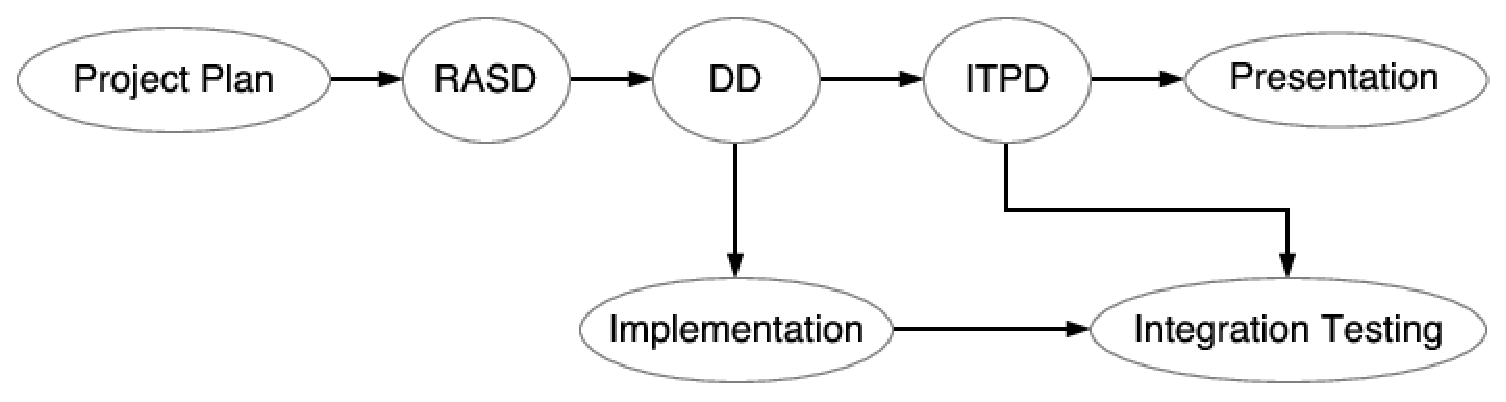
\includegraphics[width=\linewidth,keepaspectratio]{figures/dag_tasks.eps}
	\caption{DAG for the dependencies among tasks}
	\label{fig:dag_tasks}
\end{figure}

There are no fixed deadlines, instead, for the development of the software. Based on the COCOMO estimation performed in chapter 2, we expect the entire project to last 8 months, so it will be presumably finished by June 2017. The schedule for our project is outlined in table~\ref{tab:schedule}, while figure~\ref{fig:gantt} shows the Gantt chart for PowerEnJoy.

\begin{table}[H]
	\centering
	\begin{tabular}{|l|r|r|}
		\hline
		\textbf{Activity} & \textbf{Start date} & \textbf{Deadline} \\
		\hline
		RASD & 16/10/2016 & 13/11/2016 \\
		DD & 14/11/2016 & 11/12/2016 \\
		IPTD & 12/12/2016 & 15/01/2017 \\
		Project Plan & 05/01/2017 & 22/01/2017 \\
		Presentation &  &  \\
		Implementation &   &  \\
		Integration testing &   &  \\
		\hline	
	\end{tabular}

	\caption{Schedule for the project tasks}
	\label{tab:schedule}
\end{table}

\begin{figure}[H]
	\centering
	\begin{sideways}	
		\begin{ganttchart}[
			vgrid={*{6}{draw=none},dotted},
			time slot format=isodate,
			x unit=0.7mm,
			today=2017-01-22,
			today rule/.style= {ultra thick},
			today label=Today,
			link bulge=6, link tolerance=5,
			bar inline label node/.style={font=\scriptsize},
			inline
			]{2016-10-01}{2017-06-30}
			\gantttitlecalendar{year,month=name} \\
			\ganttbar[name=rasd]{RASD}{2016-10-16}{2016-11-13} \\
			\ganttbar[name=dd]{DD}{2016-11-14}{2016-12-11} \\
			\ganttbar[name=itpd]{ITPD}{2016-12-12}{2017-01-15} \\
			\ganttbar[name=pp]{PP}{2017-01-05}{2017-01-22} \\
			\ganttbar[name=pres]{Presentation}{2017-01-24}{2017-02-18} \\
			\ganttbar[name=impl]{Implementation}{2017-02-19}{2017-06-01} \\
			\ganttbar[name=int-test]{Int. Test.}{2017-06-01}{2017-06-20}
			\ganttlink{rasd}{dd}
			\ganttlink{dd}{itpd}
			\ganttlink{impl}{int-test}
		\end{ganttchart}
	\end{sideways}

	\caption{Gantt chart of the project}
	\label{fig:gantt}
\end{figure}

\end{document}
